\documentclass[10pt,twocolumn]{article}
\usepackage[margin=0.75in,columnsep=0.25in]{geometry}
\usepackage{graphicx,booktabs,amsmath,amssymb,caption,url}
\usepackage[colorlinks=true,linkcolor=blue,citecolor=blue,urlcolor=blue]{hyperref}
\captionsetup{font=small,labelfont=bf}
\setlength{\parskip}{2pt}
% AUTO-GENERATED by scripts/05_make_latex.py -- do not edit
\newcommand{\ABM}{0.596}
\newcommand{\ABMSd}{0.026}
\newcommand{\ABMacc}{35.0}
\newcommand{\AHyb}{0.691}
\newcommand{\AHybSd}{0.035}
\newcommand{\AHybacc}{57.0}
\newcommand{\ALR}{0.812}
\newcommand{\ALRSd}{0.013}
\newcommand{\ALRacc}{82.7}
\newcommand{\ATFd}{0.589}
\newcommand{\ATFdSd}{0.027}
\newcommand{\ATFdacc}{35.1}
\newcommand{\AnIn}{3,398}
\newcommand{\AnOut}{1,408}
\newcommand{\BBMTFd}{-0.6}
\newcommand{\BBMTFdHi}{-0.1}
\newcommand{\BBMTFdLo}{-1.1}
\newcommand{\BHybBM}{+21.1}
\newcommand{\BHybBMHi}{+22.6}
\newcommand{\BHybBMLo}{+19.6}
\newcommand{\BLRHyb}{+26.1}
\newcommand{\BLRHybHi}{+27.7}
\newcommand{\BLRHybLo}{+24.6}
\newcommand{\DafterAmbig}{20,536}
\newcommand{\DafterDup}{20,563}
\newcommand{\DambigRemoved}{12}
\newcommand{\DfinalRows}{20,523}
\newcommand{\DmaxQ}{1,104}
\newcommand{\DmedQ}{68}
\newcommand{\DminQ}{12}
\newcommand{\DrawRows}{20,614}
\newcommand{\Dsplittest}{4,107}
\newcommand{\Dsplittrain}{12,303}
\newcommand{\Dsplitval}{4,113}
\newcommand{\Dtools}{199}
\newcommand{\EBMNallMacro}{44.4}
\newcommand{\EBMNallMacroSd}{1.0}
\newcommand{\EBMNallMrr}{0.425}
\newcommand{\EBMNallMrrSd}{0.006}
\newcommand{\EBMNallThree}{46.1}
\newcommand{\EBMNallThreeSd}{0.3}
\newcommand{\EBMNallTop}{34.4}
\newcommand{\EBMNallTopSd}{0.9}
\newcommand{\EBMNfiftyMacro}{56.1}
\newcommand{\EBMNfiftyMacroSd}{4.0}
\newcommand{\EBMNfiftyMrr}{0.551}
\newcommand{\EBMNfiftyMrrSd}{0.065}
\newcommand{\EBMNfiftyThree}{58.8}
\newcommand{\EBMNfiftyThreeSd}{6.9}
\newcommand{\EBMNfiftyTop}{46.3}
\newcommand{\EBMNfiftyTopSd}{7.2}
\newcommand{\EBMNhundredMacro}{49.3}
\newcommand{\EBMNhundredMacroSd}{3.9}
\newcommand{\EBMNhundredMrr}{0.482}
\newcommand{\EBMNhundredMrrSd}{0.020}
\newcommand{\EBMNhundredThree}{52.2}
\newcommand{\EBMNhundredThreeSd}{2.3}
\newcommand{\EBMNhundredTop}{39.3}
\newcommand{\EBMNhundredTopSd}{1.9}
\newcommand{\EBMNtenMacro}{64.5}
\newcommand{\EBMNtenMacroSd}{8.1}
\newcommand{\EBMNtenMrr}{0.715}
\newcommand{\EBMNtenMrrSd}{0.059}
\newcommand{\EBMNtenThree}{74.1}
\newcommand{\EBMNtenThreeSd}{5.4}
\newcommand{\EBMNtenTop}{61.7}
\newcommand{\EBMNtenTopSd}{7.8}
\newcommand{\EBMNtwentyfiveMacro}{55.7}
\newcommand{\EBMNtwentyfiveMacroSd}{3.9}
\newcommand{\EBMNtwentyfiveMrr}{0.586}
\newcommand{\EBMNtwentyfiveMrrSd}{0.057}
\newcommand{\EBMNtwentyfiveThree}{62.0}
\newcommand{\EBMNtwentyfiveThreeSd}{6.2}
\newcommand{\EBMNtwentyfiveTop}{49.0}
\newcommand{\EBMNtwentyfiveTopSd}{6.5}
\newcommand{\EHybNallMacro}{63.4}
\newcommand{\EHybNallMacroSd}{0.6}
\newcommand{\EHybNallMrr}{0.643}
\newcommand{\EHybNallMrrSd}{0.006}
\newcommand{\EHybNallThree}{70.3}
\newcommand{\EHybNallThreeSd}{0.6}
\newcommand{\EHybNallTop}{54.7}
\newcommand{\EHybNallTopSd}{0.6}
\newcommand{\EHybNfiftyMacro}{75.3}
\newcommand{\EHybNfiftyMacroSd}{2.9}
\newcommand{\EHybNfiftyMrr}{0.752}
\newcommand{\EHybNfiftyMrrSd}{0.052}
\newcommand{\EHybNfiftyThree}{80.7}
\newcommand{\EHybNfiftyThreeSd}{4.9}
\newcommand{\EHybNfiftyTop}{66.8}
\newcommand{\EHybNfiftyTopSd}{6.6}
\newcommand{\EHybNhundredMacro}{69.8}
\newcommand{\EHybNhundredMacroSd}{2.3}
\newcommand{\EHybNhundredMrr}{0.707}
\newcommand{\EHybNhundredMrrSd}{0.020}
\newcommand{\EHybNhundredThree}{76.6}
\newcommand{\EHybNhundredThreeSd}{2.4}
\newcommand{\EHybNhundredTop}{61.9}
\newcommand{\EHybNhundredTopSd}{1.8}
\newcommand{\EHybNtenMacro}{87.1}
\newcommand{\EHybNtenMacroSd}{3.5}
\newcommand{\EHybNtenMrr}{0.903}
\newcommand{\EHybNtenMrrSd}{0.036}
\newcommand{\EHybNtenThree}{94.0}
\newcommand{\EHybNtenThreeSd}{2.8}
\newcommand{\EHybNtenTop}{85.3}
\newcommand{\EHybNtenTopSd}{4.9}
\newcommand{\EHybNtwentyfiveMacro}{74.5}
\newcommand{\EHybNtwentyfiveMacroSd}{3.8}
\newcommand{\EHybNtwentyfiveMrr}{0.767}
\newcommand{\EHybNtwentyfiveMrrSd}{0.055}
\newcommand{\EHybNtwentyfiveThree}{82.0}
\newcommand{\EHybNtwentyfiveThreeSd}{6.2}
\newcommand{\EHybNtwentyfiveTop}{68.6}
\newcommand{\EHybNtwentyfiveTopSd}{6.3}
\newcommand{\ELRNallMacro}{76.5}
\newcommand{\ELRNallMacroSd}{0.7}
\newcommand{\ELRNallMrr}{0.865}
\newcommand{\ELRNallMrrSd}{0.004}
\newcommand{\ELRNallThree}{91.4}
\newcommand{\ELRNallThreeSd}{0.5}
\newcommand{\ELRNallTop}{80.3}
\newcommand{\ELRNallTopSd}{0.5}
\newcommand{\ELRNfiftyMacro}{86.1}
\newcommand{\ELRNfiftyMacroSd}{2.6}
\newcommand{\ELRNfiftyMrr}{0.932}
\newcommand{\ELRNfiftyMrrSd}{0.009}
\newcommand{\ELRNfiftyThree}{96.6}
\newcommand{\ELRNfiftyThreeSd}{0.4}
\newcommand{\ELRNfiftyTop}{89.4}
\newcommand{\ELRNfiftyTopSd}{1.8}
\newcommand{\ELRNhundredMacro}{82.4}
\newcommand{\ELRNhundredMacroSd}{2.3}
\newcommand{\ELRNhundredMrr}{0.905}
\newcommand{\ELRNhundredMrrSd}{0.015}
\newcommand{\ELRNhundredThree}{94.6}
\newcommand{\ELRNhundredThreeSd}{1.3}
\newcommand{\ELRNhundredTop}{85.7}
\newcommand{\ELRNhundredTopSd}{2.0}
\newcommand{\ELRNtenMacro}{92.0}
\newcommand{\ELRNtenMacroSd}{5.3}
\newcommand{\ELRNtenMrr}{0.973}
\newcommand{\ELRNtenMrrSd}{0.016}
\newcommand{\ELRNtenThree}{99.1}
\newcommand{\ELRNtenThreeSd}{0.8}
\newcommand{\ELRNtenTop}{95.4}
\newcommand{\ELRNtenTopSd}{2.6}
\newcommand{\ELRNtwentyfiveMacro}{84.6}
\newcommand{\ELRNtwentyfiveMacroSd}{1.9}
\newcommand{\ELRNtwentyfiveMrr}{0.932}
\newcommand{\ELRNtwentyfiveMrrSd}{0.013}
\newcommand{\ELRNtwentyfiveThree}{96.4}
\newcommand{\ELRNtwentyfiveThreeSd}{1.0}
\newcommand{\ELRNtwentyfiveTop}{89.3}
\newcommand{\ELRNtwentyfiveTopSd}{2.0}
\newcommand{\ERandNallMacro}{0.5}
\newcommand{\ERandNallMacroSd}{0.0}
\newcommand{\ERandNallMrr}{0.030}
\newcommand{\ERandNallMrrSd}{0.002}
\newcommand{\ERandNallThree}{1.5}
\newcommand{\ERandNallThreeSd}{0.3}
\newcommand{\ERandNallTop}{0.5}
\newcommand{\ERandNallTopSd}{0.1}
\newcommand{\ERandNfiftyMacro}{2.1}
\newcommand{\ERandNfiftyMacroSd}{0.6}
\newcommand{\ERandNfiftyMrr}{0.091}
\newcommand{\ERandNfiftyMrrSd}{0.007}
\newcommand{\ERandNfiftyThree}{6.1}
\newcommand{\ERandNfiftyThreeSd}{0.8}
\newcommand{\ERandNfiftyTop}{2.1}
\newcommand{\ERandNfiftyTopSd}{0.5}
\newcommand{\ERandNhundredMacro}{1.2}
\newcommand{\ERandNhundredMacroSd}{0.2}
\newcommand{\ERandNhundredMrr}{0.053}
\newcommand{\ERandNhundredMrrSd}{0.002}
\newcommand{\ERandNhundredThree}{3.0}
\newcommand{\ERandNhundredThreeSd}{0.5}
\newcommand{\ERandNhundredTop}{1.1}
\newcommand{\ERandNhundredTopSd}{0.2}
\newcommand{\ERandNtenMacro}{10.6}
\newcommand{\ERandNtenMacroSd}{1.7}
\newcommand{\ERandNtenMrr}{0.305}
\newcommand{\ERandNtenMrrSd}{0.021}
\newcommand{\ERandNtenThree}{32.0}
\newcommand{\ERandNtenThreeSd}{2.3}
\newcommand{\ERandNtenTop}{10.6}
\newcommand{\ERandNtenTopSd}{2.3}
\newcommand{\ERandNtwentyfiveMacro}{3.4}
\newcommand{\ERandNtwentyfiveMacroSd}{0.6}
\newcommand{\ERandNtwentyfiveMrr}{0.151}
\newcommand{\ERandNtwentyfiveMrrSd}{0.009}
\newcommand{\ERandNtwentyfiveThree}{11.9}
\newcommand{\ERandNtwentyfiveThreeSd}{1.6}
\newcommand{\ERandNtwentyfiveTop}{3.8}
\newcommand{\ERandNtwentyfiveTopSd}{0.8}
\newcommand{\ETFdNallMacro}{44.4}
\newcommand{\ETFdNallMacroSd}{1.0}
\newcommand{\ETFdNallMrr}{0.429}
\newcommand{\ETFdNallMrrSd}{0.006}
\newcommand{\ETFdNallThree}{46.6}
\newcommand{\ETFdNallThreeSd}{0.4}
\newcommand{\ETFdNallTop}{34.7}
\newcommand{\ETFdNallTopSd}{0.9}
\newcommand{\ETFdNfiftyMacro}{55.4}
\newcommand{\ETFdNfiftyMacroSd}{4.3}
\newcommand{\ETFdNfiftyMrr}{0.549}
\newcommand{\ETFdNfiftyMrrSd}{0.067}
\newcommand{\ETFdNfiftyThree}{59.1}
\newcommand{\ETFdNfiftyThreeSd}{7.2}
\newcommand{\ETFdNfiftyTop}{45.8}
\newcommand{\ETFdNfiftyTopSd}{7.5}
\newcommand{\ETFdNhundredMacro}{49.2}
\newcommand{\ETFdNhundredMacroSd}{3.9}
\newcommand{\ETFdNhundredMrr}{0.483}
\newcommand{\ETFdNhundredMrrSd}{0.018}
\newcommand{\ETFdNhundredThree}{52.5}
\newcommand{\ETFdNhundredThreeSd}{2.3}
\newcommand{\ETFdNhundredTop}{39.5}
\newcommand{\ETFdNhundredTopSd}{1.6}
\newcommand{\ETFdNtenMacro}{65.3}
\newcommand{\ETFdNtenMacroSd}{7.7}
\newcommand{\ETFdNtenMrr}{0.717}
\newcommand{\ETFdNtenMrrSd}{0.058}
\newcommand{\ETFdNtenThree}{74.2}
\newcommand{\ETFdNtenThreeSd}{5.3}
\newcommand{\ETFdNtenTop}{62.2}
\newcommand{\ETFdNtenTopSd}{7.6}
\newcommand{\ETFdNtwentyfiveMacro}{55.7}
\newcommand{\ETFdNtwentyfiveMacroSd}{3.7}
\newcommand{\ETFdNtwentyfiveMrr}{0.587}
\newcommand{\ETFdNtwentyfiveMrrSd}{0.056}
\newcommand{\ETFdNtwentyfiveThree}{62.3}
\newcommand{\ETFdNtwentyfiveThreeSd}{6.2}
\newcommand{\ETFdNtwentyfiveTop}{49.1}
\newcommand{\ETFdNtwentyfiveTopSd}{6.4}
\newcommand{\FBMFit}{0.008}
\newcommand{\FBMMs}{0.35}
\newcommand{\FHybFit}{0.027}
\newcommand{\FHybMs}{0.47}
\newcommand{\FLRFit}{24.425}
\newcommand{\FLRMs}{0.53}
\newcommand{\FTFdFit}{0.010}
\newcommand{\FTFdMs}{0.35}
\newcommand{\Kkfiveseen}{54.1}
\newcommand{\KkfiveseenSd}{1.4}
\newcommand{\Kkfiveunseen}{42.5}
\newcommand{\KkfiveunseenSd}{4.9}
\newcommand{\Kkoneseen}{40.4}
\newcommand{\KkoneseenSd}{1.3}
\newcommand{\Kkoneunseen}{40.4}
\newcommand{\KkoneunseenSd}{3.8}
\newcommand{\Kktenseen}{60.8}
\newcommand{\KktenseenSd}{1.9}
\newcommand{\Kktenunseen}{42.6}
\newcommand{\KktenunseenSd}{4.0}
\newcommand{\Kkthreeseen}{48.7}
\newcommand{\KkthreeseenSd}{1.6}
\newcommand{\Kkthreeunseen}{42.5}
\newcommand{\KkthreeunseenSd}{3.3}
\newcommand{\Kktwentyseen}{66.1}
\newcommand{\KktwentyseenSd}{0.9}
\newcommand{\Kktwentyunseen}{43.4}
\newcommand{\KktwentyunseenSd}{4.7}
\newcommand{\Kkzeroseen}{33.8}
\newcommand{\KkzeroseenSd}{1.2}
\newcommand{\Kkzerounseen}{39.2}
\newcommand{\KkzerounseenSd}{3.2}
\newcommand{\PBMnBMseen}{+3.9}
\newcommand{\PBMnBMseenPos}{5}
\newcommand{\PBMnBMseenSd}{0.5}
\newcommand{\PBMnBMunseen}{+4.3}
\newcommand{\PBMnBMunseenPos}{5}
\newcommand{\PBMnBMunseenSd}{3.6}
\newcommand{\PHybTFdseen}{+20.3}
\newcommand{\PHybTFdseenPos}{5}
\newcommand{\PHybTFdseenSd}{0.6}
\newcommand{\PHybTFdunseen}{+3.3}
\newcommand{\PHybTFdunseenPos}{5}
\newcommand{\PHybTFdunseenSd}{1.8}
\newcommand{\PTFnTFdseen}{+4.9}
\newcommand{\PTFnTFdseenPos}{5}
\newcommand{\PTFnTFdseenSd}{0.6}
\newcommand{\PTFnTFdunseen}{+4.7}
\newcommand{\PTFnTFdunseenPos}{5}
\newcommand{\PTFnTFdunseenSd}{3.7}
\newcommand{\SBMcfivepFiftyAbs}{0.001}
\newcommand{\SBMcfivepFiftyAll}{-3.949}
\newcommand{\SBMcfivepFiftyCovIn}{3.4}
\newcommand{\SBMcfivepFiftyCovOut}{0.4}
\newcommand{\SBMcfivepFiftySel}{94.7}
\newcommand{\SBMcfivepTenAbs}{0.024}
\newcommand{\SBMcfivepTenAll}{-3.108}
\newcommand{\SBMcfivepTenCovIn}{7.6}
\newcommand{\SBMcfivepTenCovOut}{1.3}
\newcommand{\SBMcfivepTenSel}{90.9}
\newcommand{\SBMcfivepThirtyAbs}{0.011}
\newcommand{\SBMcfivepThirtyAll}{-3.529}
\newcommand{\SBMcfivepThirtyCovIn}{5.3}
\newcommand{\SBMcfivepThirtyCovOut}{0.6}
\newcommand{\SBMcfivepThirtySel}{93.3}
\newcommand{\SBMchalfpFiftyAbs}{0.041}
\newcommand{\SBMchalfpFiftyAll}{-0.237}
\newcommand{\SBMchalfpFiftyCovIn}{21.7}
\newcommand{\SBMchalfpFiftyCovOut}{10.0}
\newcommand{\SBMchalfpFiftySel}{74.1}
\newcommand{\SBMchalfpTenAbs}{0.124}
\newcommand{\SBMchalfpTenAll}{-0.027}
\newcommand{\SBMchalfpTenCovIn}{32.4}
\newcommand{\SBMchalfpTenCovOut}{19.2}
\newcommand{\SBMchalfpTenSel}{64.2}
\newcommand{\SBMchalfpThirtyAbs}{0.079}
\newcommand{\SBMchalfpThirtyAll}{-0.132}
\newcommand{\SBMchalfpThirtyCovIn}{25.8}
\newcommand{\SBMchalfpThirtyCovOut}{13.3}
\newcommand{\SBMchalfpThirtySel}{70.3}
\newcommand{\SBMconepFiftyAbs}{0.025}
\newcommand{\SBMconepFiftyAll}{-0.650}
\newcommand{\SBMconepFiftyCovIn}{11.9}
\newcommand{\SBMconepFiftyCovOut}{3.5}
\newcommand{\SBMconepFiftySel}{85.7}
\newcommand{\SBMconepTenAbs}{0.084}
\newcommand{\SBMconepTenAll}{-0.369}
\newcommand{\SBMconepTenCovIn}{21.3}
\newcommand{\SBMconepTenCovOut}{9.5}
\newcommand{\SBMconepTenSel}{74.6}
\newcommand{\SBMconepThirtyAbs}{0.046}
\newcommand{\SBMconepThirtyAll}{-0.510}
\newcommand{\SBMconepThirtyCovIn}{17.6}
\newcommand{\SBMconepThirtyCovOut}{6.9}
\newcommand{\SBMconepThirtySel}{77.6}
\newcommand{\SBMctwopFiftyAbs}{0.009}
\newcommand{\SBMctwopFiftyAll}{-1.475}
\newcommand{\SBMctwopFiftyCovIn}{8.7}
\newcommand{\SBMctwopFiftyCovOut}{2.1}
\newcommand{\SBMctwopFiftySel}{89.8}
\newcommand{\SBMctwopTenAbs}{0.052}
\newcommand{\SBMctwopTenAll}{-1.054}
\newcommand{\SBMctwopTenCovIn}{12.2}
\newcommand{\SBMctwopTenCovOut}{3.6}
\newcommand{\SBMctwopTenSel}{84.7}
\newcommand{\SBMctwopThirtyAbs}{0.029}
\newcommand{\SBMctwopThirtyAll}{-1.264}
\newcommand{\SBMctwopThirtyCovIn}{9.6}
\newcommand{\SBMctwopThirtyCovOut}{2.4}
\newcommand{\SBMctwopThirtySel}{88.4}
\newcommand{\SBMczeropFiftyAbs}{0.175}
\newcommand{\SBMczeropFiftyAll}{0.175}
\newcommand{\SBMczeropFiftyCovIn}{100.0}
\newcommand{\SBMczeropFiftyCovOut}{100.0}
\newcommand{\SBMczeropFiftySel}{35.0}
\newcommand{\SBMczeropTenAbs}{0.315}
\newcommand{\SBMczeropTenAll}{0.315}
\newcommand{\SBMczeropTenCovIn}{100.0}
\newcommand{\SBMczeropTenCovOut}{100.0}
\newcommand{\SBMczeropTenSel}{35.0}
\newcommand{\SBMczeropThirtyAbs}{0.245}
\newcommand{\SBMczeropThirtyAll}{0.245}
\newcommand{\SBMczeropThirtyCovIn}{100.0}
\newcommand{\SBMczeropThirtyCovOut}{100.0}
\newcommand{\SBMczeropThirtySel}{35.0}
\newcommand{\SHybcfivepFiftyAbs}{0.010}
\newcommand{\SHybcfivepFiftyAll}{-3.291}
\newcommand{\SHybcfivepFiftyCovIn}{8.5}
\newcommand{\SHybcfivepFiftyCovOut}{1.0}
\newcommand{\SHybcfivepFiftySel}{97.7}
\newcommand{\SHybcfivepTenAbs}{0.086}
\newcommand{\SHybcfivepTenAll}{-1.923}
\newcommand{\SHybcfivepTenCovIn}{18.6}
\newcommand{\SHybcfivepTenCovOut}{3.7}
\newcommand{\SHybcfivepTenSel}{93.7}
\newcommand{\SHybcfivepThirtyAbs}{0.034}
\newcommand{\SHybcfivepThirtyAll}{-2.607}
\newcommand{\SHybcfivepThirtyCovIn}{13.7}
\newcommand{\SHybcfivepThirtyCovOut}{2.2}
\newcommand{\SHybcfivepThirtySel}{95.2}
\newcommand{\SHybchalfpFiftyAbs}{0.122}
\newcommand{\SHybchalfpFiftyAll}{-0.073}
\newcommand{\SHybchalfpFiftyCovIn}{45.5}
\newcommand{\SHybchalfpFiftyCovOut}{17.9}
\newcommand{\SHybchalfpFiftySel}{82.1}
\newcommand{\SHybchalfpTenAbs}{0.330}
\newcommand{\SHybchalfpTenAll}{0.269}
\newcommand{\SHybchalfpTenCovIn}{69.7}
\newcommand{\SHybchalfpTenCovOut}{43.9}
\newcommand{\SHybchalfpTenSel}{70.8}
\newcommand{\SHybchalfpThirtyAbs}{0.216}
\newcommand{\SHybchalfpThirtyAll}{0.098}
\newcommand{\SHybchalfpThirtyCovIn}{56.6}
\newcommand{\SHybchalfpThirtyCovOut}{28.3}
\newcommand{\SHybchalfpThirtySel}{76.9}
\newcommand{\SHybconepFiftyAbs}{0.076}
\newcommand{\SHybconepFiftyAll}{-0.430}
\newcommand{\SHybconepFiftyCovIn}{34.4}
\newcommand{\SHybconepFiftyCovOut}{10.4}
\newcommand{\SHybconepFiftySel}{87.2}
\newcommand{\SHybconepTenAbs}{0.247}
\newcommand{\SHybconepTenAll}{0.026}
\newcommand{\SHybconepTenCovIn}{51.3}
\newcommand{\SHybconepTenCovOut}{23.2}
\newcommand{\SHybconepTenSel}{79.4}
\newcommand{\SHybconepThirtyAbs}{0.152}
\newcommand{\SHybconepThirtyAll}{-0.202}
\newcommand{\SHybconepThirtyCovIn}{41.9}
\newcommand{\SHybconepThirtyCovOut}{15.5}
\newcommand{\SHybconepThirtySel}{83.7}
\newcommand{\SHybctwopFiftyAbs}{0.039}
\newcommand{\SHybctwopFiftyAll}{-1.145}
\newcommand{\SHybctwopFiftyCovIn}{18.8}
\newcommand{\SHybctwopFiftyCovOut}{3.7}
\newcommand{\SHybctwopFiftySel}{93.6}
\newcommand{\SHybctwopTenAbs}{0.168}
\newcommand{\SHybctwopTenAll}{-0.462}
\newcommand{\SHybctwopTenCovIn}{37.9}
\newcommand{\SHybctwopTenCovOut}{12.4}
\newcommand{\SHybctwopTenSel}{85.7}
\newcommand{\SHybctwopThirtyAbs}{0.093}
\newcommand{\SHybctwopThirtyAll}{-0.803}
\newcommand{\SHybctwopThirtyCovIn}{25.2}
\newcommand{\SHybctwopThirtyCovOut}{5.8}
\newcommand{\SHybctwopThirtySel}{90.8}
\newcommand{\SHybczeropFiftyAbs}{0.285}
\newcommand{\SHybczeropFiftyAll}{0.285}
\newcommand{\SHybczeropFiftyCovIn}{100.0}
\newcommand{\SHybczeropFiftyCovOut}{100.0}
\newcommand{\SHybczeropFiftySel}{57.0}
\newcommand{\SHybczeropTenAbs}{0.513}
\newcommand{\SHybczeropTenAll}{0.513}
\newcommand{\SHybczeropTenCovIn}{100.0}
\newcommand{\SHybczeropTenCovOut}{100.0}
\newcommand{\SHybczeropTenSel}{57.0}
\newcommand{\SHybczeropThirtyAbs}{0.399}
\newcommand{\SHybczeropThirtyAll}{0.399}
\newcommand{\SHybczeropThirtyCovIn}{100.0}
\newcommand{\SHybczeropThirtyCovOut}{100.0}
\newcommand{\SHybczeropThirtySel}{57.0}
\newcommand{\SLRcfivepFiftyAbs}{0.002}
\newcommand{\SLRcfivepFiftyAll}{-2.519}
\newcommand{\SLRcfivepFiftyCovIn}{23.9}
\newcommand{\SLRcfivepFiftyCovOut}{4.0}
\newcommand{\SLRcfivepFiftySel}{97.9}
\newcommand{\SLRcfivepTenAbs}{0.283}
\newcommand{\SLRcfivepTenAll}{-0.534}
\newcommand{\SLRcfivepTenCovIn}{58.9}
\newcommand{\SLRcfivepTenCovOut}{15.1}
\newcommand{\SLRcfivepTenSel}{94.6}
\newcommand{\SLRcfivepThirtyAbs}{0.104}
\newcommand{\SLRcfivepThirtyAll}{-1.526}
\newcommand{\SLRcfivepThirtyCovIn}{41.7}
\newcommand{\SLRcfivepThirtyCovOut}{8.7}
\newcommand{\SLRcfivepThirtySel}{96.7}
\newcommand{\SLRchalfpFiftyAbs}{0.264}
\newcommand{\SLRchalfpFiftyAll}{0.120}
\newcommand{\SLRchalfpFiftyCovIn}{80.3}
\newcommand{\SLRchalfpFiftyCovOut}{31.1}
\newcommand{\SLRchalfpFiftySel}{90.1}
\newcommand{\SLRchalfpTenAbs}{0.633}
\newcommand{\SLRchalfpTenAll}{0.617}
\newcommand{\SLRchalfpTenCovIn}{93.1}
\newcommand{\SLRchalfpTenCovOut}{58.3}
\newcommand{\SLRchalfpTenSel}{86.0}
\newcommand{\SLRchalfpThirtyAbs}{0.437}
\newcommand{\SLRchalfpThirtyAll}{0.368}
\newcommand{\SLRchalfpThirtyCovIn}{87.5}
\newcommand{\SLRchalfpThirtyCovOut}{43.4}
\newcommand{\SLRchalfpThirtySel}{88.0}
\newcommand{\SLRconepFiftyAbs}{0.190}
\newcommand{\SLRconepFiftyAll}{-0.173}
\newcommand{\SLRconepFiftyCovIn}{70.8}
\newcommand{\SLRconepFiftyCovOut}{22.2}
\newcommand{\SLRconepFiftySel}{92.5}
\newcommand{\SLRconepTenAbs}{0.554}
\newcommand{\SLRconepTenAll}{0.489}
\newcommand{\SLRconepTenCovIn}{88.4}
\newcommand{\SLRconepTenCovOut}{45.4}
\newcommand{\SLRconepTenSel}{87.7}
\newcommand{\SLRconepThirtyAbs}{0.359}
\newcommand{\SLRconepThirtyAll}{0.158}
\newcommand{\SLRconepThirtyCovIn}{79.4}
\newcommand{\SLRconepThirtyCovOut}{30.1}
\newcommand{\SLRconepThirtySel}{90.4}
\newcommand{\SLRctwopFiftyAbs}{0.103}
\newcommand{\SLRctwopFiftyAll}{-0.759}
\newcommand{\SLRctwopFiftyCovIn}{53.1}
\newcommand{\SLRctwopFiftyCovOut}{12.7}
\newcommand{\SLRctwopFiftySel}{95.6}
\newcommand{\SLRctwopTenAbs}{0.450}
\newcommand{\SLRctwopTenAll}{0.233}
\newcommand{\SLRctwopTenCovIn}{74.1}
\newcommand{\SLRctwopTenCovOut}{24.9}
\newcommand{\SLRctwopTenSel}{91.7}
\newcommand{\SLRctwopThirtyAbs}{0.258}
\newcommand{\SLRctwopThirtyAll}{-0.263}
\newcommand{\SLRctwopThirtyCovIn}{65.4}
\newcommand{\SLRctwopThirtyCovOut}{18.5}
\newcommand{\SLRctwopThirtySel}{93.5}
\newcommand{\SLRczeropFiftyAbs}{0.414}
\newcommand{\SLRczeropFiftyAll}{0.414}
\newcommand{\SLRczeropFiftyCovIn}{100.0}
\newcommand{\SLRczeropFiftyCovOut}{100.0}
\newcommand{\SLRczeropFiftySel}{82.7}
\newcommand{\SLRczeropTenAbs}{0.744}
\newcommand{\SLRczeropTenAll}{0.744}
\newcommand{\SLRczeropTenCovIn}{100.0}
\newcommand{\SLRczeropTenCovOut}{100.0}
\newcommand{\SLRczeropTenSel}{82.7}
\newcommand{\SLRczeropThirtyAbs}{0.579}
\newcommand{\SLRczeropThirtyAll}{0.579}
\newcommand{\SLRczeropThirtyCovIn}{100.0}
\newcommand{\SLRczeropThirtyCovOut}{100.0}
\newcommand{\SLRczeropThirtySel}{82.7}
\newcommand{\STFdcfivepFiftyAbs}{0.002}
\newcommand{\STFdcfivepFiftyAll}{-3.946}
\newcommand{\STFdcfivepFiftyCovIn}{2.1}
\newcommand{\STFdcfivepFiftyCovOut}{0.3}
\newcommand{\STFdcfivepFiftySel}{96.4}
\newcommand{\STFdcfivepTenAbs}{0.021}
\newcommand{\STFdcfivepTenAll}{-3.102}
\newcommand{\STFdcfivepTenCovIn}{6.7}
\newcommand{\STFdcfivepTenCovOut}{1.8}
\newcommand{\STFdcfivepTenSel}{91.6}
\newcommand{\STFdcfivepThirtyAbs}{0.004}
\newcommand{\STFdcfivepThirtyAll}{-3.524}
\newcommand{\STFdcfivepThirtyCovIn}{4.5}
\newcommand{\STFdcfivepThirtyCovOut}{1.0}
\newcommand{\STFdcfivepThirtySel}{93.6}
\newcommand{\STFdchalfpFiftyAbs}{0.036}
\newcommand{\STFdchalfpFiftyAll}{-0.236}
\newcommand{\STFdchalfpFiftyCovIn}{20.8}
\newcommand{\STFdchalfpFiftyCovOut}{10.5}
\newcommand{\STFdchalfpFiftySel}{74.1}
\newcommand{\STFdchalfpTenAbs}{0.123}
\newcommand{\STFdchalfpTenAll}{-0.026}
\newcommand{\STFdchalfpTenCovIn}{38.9}
\newcommand{\STFdchalfpTenCovOut}{26.5}
\newcommand{\STFdchalfpTenSel}{60.2}
\newcommand{\STFdchalfpThirtyAbs}{0.078}
\newcommand{\STFdchalfpThirtyAll}{-0.131}
\newcommand{\STFdchalfpThirtyCovIn}{26.9}
\newcommand{\STFdchalfpThirtyCovOut}{14.6}
\newcommand{\STFdchalfpThirtySel}{68.7}
\newcommand{\STFdconepFiftyAbs}{0.023}
\newcommand{\STFdconepFiftyAll}{-0.649}
\newcommand{\STFdconepFiftyCovIn}{9.3}
\newcommand{\STFdconepFiftyCovOut}{2.5}
\newcommand{\STFdconepFiftySel}{88.6}
\newcommand{\STFdconepTenAbs}{0.078}
\newcommand{\STFdconepTenAll}{-0.367}
\newcommand{\STFdconepTenCovIn}{22.8}
\newcommand{\STFdconepTenCovOut}{11.5}
\newcommand{\STFdconepTenSel}{71.8}
\newcommand{\STFdconepThirtyAbs}{0.045}
\newcommand{\STFdconepThirtyAll}{-0.508}
\newcommand{\STFdconepThirtyCovIn}{14.9}
\newcommand{\STFdconepThirtyCovOut}{6.0}
\newcommand{\STFdconepThirtySel}{80.2}
\newcommand{\STFdctwopFiftyAbs}{0.009}
\newcommand{\STFdctwopFiftyAll}{-1.473}
\newcommand{\STFdctwopFiftyCovIn}{7.3}
\newcommand{\STFdctwopFiftyCovOut}{1.9}
\newcommand{\STFdctwopFiftySel}{91.2}
\newcommand{\STFdctwopTenAbs}{0.044}
\newcommand{\STFdctwopTenAll}{-1.051}
\newcommand{\STFdctwopTenCovIn}{11.4}
\newcommand{\STFdctwopTenCovOut}{4.0}
\newcommand{\STFdctwopTenSel}{85.1}
\newcommand{\STFdctwopThirtyAbs}{0.026}
\newcommand{\STFdctwopThirtyAll}{-1.262}
\newcommand{\STFdctwopThirtyCovIn}{8.9}
\newcommand{\STFdctwopThirtyCovOut}{2.5}
\newcommand{\STFdctwopThirtySel}{89.1}
\newcommand{\STFdczeropFiftyAbs}{0.176}
\newcommand{\STFdczeropFiftyAll}{0.176}
\newcommand{\STFdczeropFiftyCovIn}{100.0}
\newcommand{\STFdczeropFiftyCovOut}{100.0}
\newcommand{\STFdczeropFiftySel}{35.1}
\newcommand{\STFdczeropTenAbs}{0.316}
\newcommand{\STFdczeropTenAll}{0.316}
\newcommand{\STFdczeropTenCovIn}{100.0}
\newcommand{\STFdczeropTenCovOut}{100.0}
\newcommand{\STFdczeropTenSel}{35.1}
\newcommand{\STFdczeropThirtyAbs}{0.246}
\newcommand{\STFdczeropThirtyAll}{0.246}
\newcommand{\STFdczeropThirtyCovIn}{100.0}
\newcommand{\STFdczeropThirtyCovOut}{100.0}
\newcommand{\STFdczeropThirtySel}{35.1}
\newcommand{\TBMnseen}{37.5}
\newcommand{\TBMnseenSd}{1.5}
\newcommand{\TBMnunseen}{43.1}
\newcommand{\TBMnunseenSd}{5.7}
\newcommand{\TBMseen}{33.6}
\newcommand{\TBMseenSd}{1.3}
\newcommand{\TBMunseen}{38.8}
\newcommand{\TBMunseenSd}{2.9}
\newcommand{\THybnseen}{55.4}
\newcommand{\THybnseenSd}{1.4}
\newcommand{\THybnunseen}{45.2}
\newcommand{\THybnunseenSd}{7.4}
\newcommand{\THybseen}{54.1}
\newcommand{\THybseenSd}{1.4}
\newcommand{\THybunseen}{42.5}
\newcommand{\THybunseenSd}{4.9}
\newcommand{\TLRseen}{82.7}
\newcommand{\TLRseenSd}{0.7}
\newcommand{\TLRunseen}{0.0}
\newcommand{\TLRunseenSd}{0.0}
\newcommand{\TTFdseen}{33.8}
\newcommand{\TTFdseenSd}{1.2}
\newcommand{\TTFdunseen}{39.2}
\newcommand{\TTFdunseenSd}{3.2}
\newcommand{\TTFnseen}{38.7}
\newcommand{\TTFnseenSd}{1.3}
\newcommand{\TTFnunseen}{43.9}
\newcommand{\TTFnunseenSd}{5.9}
\newcommand{\VbmDiff}{7.1\times 10^{-15}}
\newcommand{\VchanceTop}{0.5}
\newcommand{\VrandTop}{0.4}
\newcommand{\VselC}{10}
\newcommand{\VshufMacro}{0.3}
\newcommand{\VshufTop}{1.7}
\newcommand{\VvalCI}{71.2}
\newcommand{\VvalCIO}{80.5}
\newcommand{\VvalCIOO}{80.3}
\newcommand{\XBMErr}{13,471}
\newcommand{\XBMMacroPt}{44.4}
\newcommand{\XBMMicro}{34.4}
\newcommand{\XBMSpear}{-0.18}
\newcommand{\XBMTopShare}{8.5}
\newcommand{\XHybErr}{9,301}
\newcommand{\XHybMacroPt}{63.4}
\newcommand{\XHybMicro}{54.7}
\newcommand{\XHybSpear}{-0.11}
\newcommand{\XHybTopShare}{10.7}
\newcommand{\XLRErr}{4,043}
\newcommand{\XLRMacroPt}{76.5}
\newcommand{\XLRMicro}{80.3}
\newcommand{\XLRSpear}{+0.20}
\newcommand{\XLRTopShare}{17.2}

\title{\vspace{-0.4in}\textbf{How Far Do Simple Selectors Go? Library Scale, Unseen Tools and Cost-Aware Abstention in Tool Selection on MetaTool}}
\author{Dhairya Ashvinbhai Prajapati\\ Networks Systems and Computing (Roll No.\ MNS2026005), India}
\date{}
\begin{document}\maketitle\vspace{-0.2in}
\begin{abstract}
My earlier literature review~(\emph{Evaluating Tool-Selection Accuracy in Multi-Tool Agentic AI Systems}) organised tool selection into four strategies and argued that (i) large tool libraries break context-based selection, (ii) fine-tuned selectors suffer on unseen tools, and (iii) top-1 accuracy overstates reliability, motivating a cost-adjusted score. It tested none of this. Here I run a controlled comparative study on the MetaTool ToolE single-tool queries (\Dtools{} tools, \DfinalRows{} cleaned queries) with two lexical retrieval baselines (BM25, TF-IDF), an exemplar-augmented retrieval hybrid, and a supervised TF-IDF$+$logistic-regression selector as a lightweight analogue of fine-tuned selection. \emph{No LLM is evaluated.} Over five seeds: (1) accuracy falls with library size for every method, e.g.\ description-only retrieval from \EBMNtenTop\% ($N{=}10$) to \EBMNallTop\% ($N{=}199$) and the supervised selector from \ELRNtenTop\% to \ELRNallTop\%; (2) the supervised selector cannot select a tool it was not trained on (\TLRunseen\% by construction), whereas adding a few training queries to retrieval documents lifts seen-tool accuracy to \THybseen\% and gives a small paired gain of \PHybTFdunseen\,pp on unseen tools; (3) with an operational cost-adjusted score (EAS), method \emph{ranking} is unchanged relative to accuracy for $c\le2$, but answering every query yields negative scores once a wrong selection costs $c\ge1$ and raw confidence separates in-library from out-of-library queries only moderately (AUROC \ABM--\ALR{} across methods). Error analysis shows that many remaining errors are between near-duplicate tools. All code, logs and a frozen protocol are provided.
\end{abstract}

\section{Introduction}
Tool selection is the bridge between abstract task plans and grounded execution in LLM agents, and it is where agent loops commonly fail~\cite{qu2025toollearning}. My review surveyed in-context, reasoning-based, fine-tuned and retrieval-based selection strategies (ReAct~\cite{yao2023react}, Gorilla~\cite{patil2023gorilla}, ToolLLM~\cite{qin2023toolllm}, AnyTool~\cite{du2024anytool}, RestGPT~\cite{song2023restgpt}) and benchmarks such as API-Bank~\cite{li2023apibank} and MetaTool~\cite{huang2024metatool}. Its ``gaps'' section made three claims that were \emph{argued, not measured}: library scale forces retrieval; fine-tuned methods ``suffer from unseen tools''; and a cost-aware score would expose risk hidden by accuracy. This paper converts those claims into measurable questions on a public benchmark, using cheap, fully reproducible selectors so that every run can be repeated on a laptop.

\paragraph{Research questions.}
\textbf{RQ1} How does closed-set top-1 accuracy of description-only retrieval, exemplar-augmented retrieval and a supervised classifier change as the tool library grows from 10 to 199 tools? \emph{Expectation:} monotone decline; \emph{contradicted if} accuracy at $N{=}199$ is not lower than at $N{=}10$ beyond seed variation.
\textbf{RQ2} For tools without any training queries, how much accuracy can description-only or exemplar-augmented retrieval retain, and does adding exemplars for \emph{other} tools help or hurt them?
\textbf{RQ3} When the correct tool may be absent from the library, does a cost-adjusted score (EAS) change which selector looks best compared with accuracy, and how effective is confidence-based abstention?

\paragraph{Contribution (and what it is not).} This is a controlled comparative study (pathway B) with a targeted component (exemplar-augmented documents, pathway C) and a deeper analysis (ablations, sensitivity, error and efficiency analysis). It is \emph{not} a new algorithm, it does not evaluate LLM selectors, and the supervised model is a proxy for, not an instance of, LLM fine-tuning.

\section{Background and Link to the Review}
The review's taxonomy distinguishes how candidate tools are exposed to the model: in the prompt, inside a reasoning loop, through weights, or through a retriever. Retrieval-based selection narrows thousands of APIs to a few before an LLM chooses~\cite{du2024anytool,song2023restgpt}; fine-tuned selection internalises API names and arguments~\cite{patil2023gorilla,qin2023toolllm}. MetaTool~\cite{huang2024metatool} provides the ToolE queries and tool descriptions used here; per its public README the single-tool queries were generated with ChatGPT/GPT-4 (a threat to validity, Sec.~\ref{sec:limits}). My experiments use only the data files from the official repository (MIT licence; commit \texttt{35e81bb}), \emph{not} MetaTool's LLM prompts. Other claims about prior systems are repeated from my review and were not re-verified here.

\section{Method}
\paragraph{Data and cleaning.} Table~\ref{tab:data} lists each step; two issues in the raw file mattered: \DambigRemoved{} normalised query texts carry more than one gold tool, and the tool distribution is heavily imbalanced (\DminQ{} to \DmaxQ{} queries per tool), so I report macro as well as micro accuracy. Splits are per-tool stratified random (\Dsplittrain{} train / \Dsplitval{} val / \Dsplittest{} test queries per seed), after text-level de-duplication so no normalised query text appears in two splits (verified, Sec.~\ref{sec:val}).

\paragraph{Selectors.} All receive the same tool descriptions (1--2 sentences) and, where noted, training queries.
\emph{BM25}~\cite{robertson2009bm25} ($k_1{=}1.5$, $b{=}0.75$, own implementation). \emph{TF-IDF-desc}: cosine between sublinear TF-IDF vectors of query and description. \emph{Hybrid($k$)}: the same cosine retriever but each tool's document is its description plus $k{=}5$ training queries sampled for that tool (descriptions only for tools without training queries). \emph{TF-IDF+LR}: multinomial logistic regression on TF-IDF of the training queries ($C{=}\VselC$ chosen on validation data only), the fine-tuned-selection analogue. \emph{Random} is a chance control. Tokenisation and stop-word handling are shared; ties are broken randomly with a fixed seed.

\paragraph{Experiments (frozen in \texttt{configs/protocol.json}).}
\textbf{E1 (scale):} for $N\in\{10,25,50,100,199\}$ sample $N$ tools per seed, restrict train/test to them, and score top-1, top-3, MRR and macro top-1.
\textbf{E2 (unseen tools):} per seed withhold all training queries of 20\% of tools (``unseen''); the library still contains all 199 descriptions; report accuracy on test queries of seen and unseen tools separately. Sensitivity: exemplars $k\in\{0,1,3,5,10,20\}$; ablation: adding split tool-name tokens to the tool document.
\textbf{E3 (open world, EAS):} the library holds only the 159 seen tools. In-library queries are test queries of those tools; out-of-library queries are all queries of withheld tools, split into two disjoint tool groups $O_{val}$ and $O_{test}$. An abstention rule ``answer iff top-1 score $\ge\tau$'' has $\tau$ tuned on in-library validation queries $+$ $O_{val}$ queries, and evaluated on test queries $+$ $O_{test}$ queries.

\paragraph{Metrics.} Closed-set: top-1 (primary), top-3, MRR, macro top-1. Open-world: with answer indicator $a_i$ and chosen tool $t_i$,
\begin{equation}
\mathrm{EAS}_c=\tfrac1N\textstyle\sum_i\big(\mathbb 1[a_i{=}1\wedge t_i{=}t^*_i]-c\,\mathbb 1[a_i{=}1\wedge t_i{\ne}t^*_i]\big),
\end{equation}
where abstention scores 0 and any selection for an out-of-library query is wrong. It equals accuracy when $c{=}0$ and $a_i{\equiv}1$. \textbf{This deliberately differs from Eq.~(2) of my review}, which subtracts $c_i$ from every item including correct ones and whose accompanying text is ambiguous; I treat that equation as superseded. The in-library/out-of-library mix is $p_{out}{=}0.5$ (primary; 0.1 and 0.3 as sensitivity), and AUROC of the top-1 score for in- vs.\ out-of-library queries is threshold-free.

\paragraph{Reproducibility.} Seeds 0--4; \texttt{pip} versions in \texttt{requirements.txt}; one script per stage; all tables and figures are regenerated from CSVs, and the numbers in this paper are LaTeX macros produced by \texttt{scripts/05\_make\_latex.py}.

\begin{table}[t]\centering\caption{Data cleaning (script \texttt{src/data.py}). All counts are produced by the code.}\label{tab:data}\small\begin{tabular}{lr}\toprule Step & Rows\\\midrule
Raw MetaTool single-tool queries & 20,614\\
After dropping exact duplicate (query,tool) rows & 20,563\\
After dropping 12 ambiguous texts (>1 gold tool) & 20,536\\
After one-row-per-normalised-text & 20,523\\
Queries/tool (min / median / max) & 12 / 68 / 1,104\\\bottomrule\end{tabular}\end{table}

\begin{table*}[t]\centering\caption{E1: closed-set top-1 accuracy (\%), mean\,$\pm$\,s.d.\ over 5 seeds, versus library size $N$ (chance $=100/N$).}\label{tab:e1}\small\begin{tabular}{lccccc}\toprule Method & $N{=}10$ & $N{=}25$ & $N{=}50$ & $N{=}100$ & $N{=}199$\\\midrule
Random & 10.6\,$\pm$\,2.3 & 3.8\,$\pm$\,0.8 & 2.1\,$\pm$\,0.5 & 1.1\,$\pm$\,0.2 & 0.5\,$\pm$\,0.1\\
BM25 & 61.7\,$\pm$\,7.8 & 49.0\,$\pm$\,6.5 & 46.3\,$\pm$\,7.2 & 39.3\,$\pm$\,1.9 & 34.4\,$\pm$\,0.9\\
TFIDF-desc & 62.2\,$\pm$\,7.6 & 49.1\,$\pm$\,6.4 & 45.8\,$\pm$\,7.5 & 39.5\,$\pm$\,1.6 & 34.7\,$\pm$\,0.9\\
Hybrid(k=5) & 85.3\,$\pm$\,4.9 & 68.6\,$\pm$\,6.3 & 66.8\,$\pm$\,6.6 & 61.9\,$\pm$\,1.8 & 54.7\,$\pm$\,0.6\\
TFIDF+LR & 95.4\,$\pm$\,2.6 & 89.3\,$\pm$\,2.0 & 89.4\,$\pm$\,1.8 & 85.7\,$\pm$\,2.0 & 80.3\,$\pm$\,0.5\\
\bottomrule\end{tabular}\end{table*}

\begin{table}[t]\centering\caption{E1 at $N{=}199$: additional metrics (mean over 5 seeds).}\label{tab:e1b}\small\begin{tabular}{lccc}\toprule Method & Top-3 (\%) & MRR & Macro top-1 (\%)\\\midrule
BM25 & 46.1\,$\pm$\,0.3 & 0.425 & 44.4\,$\pm$\,1.0\\
TFIDF-desc & 46.6\,$\pm$\,0.4 & 0.429 & 44.4\,$\pm$\,1.0\\
Hybrid(k=5) & 70.3\,$\pm$\,0.6 & 0.643 & 63.4\,$\pm$\,0.6\\
TFIDF+LR & 91.4\,$\pm$\,0.5 & 0.865 & 76.5\,$\pm$\,0.7\\
\bottomrule\end{tabular}\end{table}

\begin{table}[t]\centering\caption{E2: top-1 (\%) over the full 199-tool library on test queries of tools whose training queries were seen / withheld ($\approx$40 tools per seed). ``+name'' appends split tool-name tokens to the tool document.}\label{tab:e2}\small\begin{tabular}{lcc}\toprule Method & Seen tools & Unseen tools\\\midrule
BM25 & 33.6\,$\pm$\,1.3 & 38.8\,$\pm$\,2.9\\
BM25+name & 37.5\,$\pm$\,1.5 & 43.1\,$\pm$\,5.7\\
TFIDF-desc & 33.8\,$\pm$\,1.2 & 39.2\,$\pm$\,3.2\\
TFIDF-desc+name & 38.7\,$\pm$\,1.3 & 43.9\,$\pm$\,5.9\\
Hybrid(k=5) & 54.1\,$\pm$\,1.4 & 42.5\,$\pm$\,4.9\\
Hybrid(k=5)+name & 55.4\,$\pm$\,1.4 & 45.2\,$\pm$\,7.4\\
TFIDF+LR & 82.7\,$\pm$\,0.7 & 0.0\,$\pm$\,0.0\\
\bottomrule\end{tabular}\end{table}

\begin{table}[t]\centering\caption{E3: EAS$_c$ at $p_{out}{=}0.5$ (mean of 5 seeds): always answering vs.\ validation-tuned abstention. Abstention gain is positive by construction of the tuning (the threshold set includes ``answer all'') but is evaluated on held-out test data.}\label{tab:e3}\small\resizebox{\columnwidth}{!}{\begin{tabular}{lcccccc}\toprule
& \multicolumn{2}{c}{$c{=}0.5$} & \multicolumn{2}{c}{$c{=}1$} & \multicolumn{2}{c}{$c{=}2$}\\ Method & answer & abstain & answer & abstain & answer & abstain\\\midrule
BM25 & -0.237 & 0.041 & -0.650 & 0.025 & -1.475 & 0.009\\
TFIDF-desc & -0.236 & 0.036 & -0.649 & 0.023 & -1.473 & 0.009\\
Hybrid(k=5) & -0.073 & 0.122 & -0.430 & 0.076 & -1.145 & 0.039\\
TFIDF+LR & 0.120 & 0.264 & -0.173 & 0.190 & -0.759 & 0.103\\
\bottomrule\end{tabular}}\end{table}

\begin{table}[t]\centering\caption{Resource use at $N{=}199$ (1 vCPU Xeon 2.1\,GHz): training/indexing time and single-query latency.}\label{tab:eff}\small\begin{tabular}{lcc}\toprule Method & Fit/index (s) & Latency (ms/query)\\\midrule
BM25 & 0.008 & 0.35\\
TFIDF-desc & 0.010 & 0.35\\
Hybrid(k=5) & 0.027 & 0.47\\
TFIDF+LR & 24.425 & 0.53\\
\bottomrule\end{tabular}\end{table}

\begin{table}[t]\centering\caption{Most frequent confusions of the supervised model (gold $\rightarrow$ predicted), pooled over 5 seeds.}\label{tab:conf}\small\begin{tabular}{llr}\toprule Gold tool & Predicted tool & Errors\\\midrule
\texttt{ResearchHelper} & \texttt{ResearchFinder} & 102\\
\texttt{ResearchFinder} & \texttt{ResearchHelper} & 80\\
\texttt{TripAdviceTool} & \texttt{TripTool} & 78\\
\texttt{TripTool} & \texttt{TripAdviceTool} & 65\\
\texttt{seoanalysis} & \texttt{SEOTool} & 37\\
\texttt{HouseRentingTool} & \texttt{HousePurchasingTool} & 30\\
\bottomrule\end{tabular}\end{table}

\section{Baseline Validation}\label{sec:val}
Before comparing methods I checked the pipeline (log: \texttt{results/baseline\_validation.json}). (a)~My BM25 agrees with the reference \texttt{rank\_bm25} implementation on 300 queries $\times$ 199 tools to a maximum absolute score difference of $\VbmDiff$. (b)~Random selection scores \VrandTop\% (chance \VchanceTop\%). (c)~A logistic-regression model trained on \emph{shuffled} labels reaches macro top-1 \VshufMacro\% (chance level) but micro top-1 \VshufTop\%, because it learns the majority-class prior; this shows why micro accuracy alone is misleading on this dataset. (d)~No normalised query text is shared between train, validation and test, and every test tool has training queries. (e)~$C{=}1,10,100$ gave validation top-1 of \VvalCI, \VvalCIO{} and \VvalCIOO\%; $C{=}\VselC$ was frozen. (f)~Metric functions pass unit checks (EAS equals accuracy at $c{=}0$ without abstention). I do not compare against published numbers because MetaTool evaluates LLMs on a different protocol; validation here establishes implementation correctness and the absence of leakage, not reproduction of a published score.

\section{Results}
\subsection{E1: library scale (RQ1)}
Table~\ref{tab:e1} and Fig.~\ref{fig:e1} show a decline for every method. Description-only BM25 drops from \EBMNtenTop\,$\pm$\,\EBMNtenTopSd\% to \EBMNallTop\,$\pm$\,\EBMNallTopSd\%; Hybrid from \EHybNtenTop\% to \EHybNallTop\%; the supervised selector from \ELRNtenTop\% to \ELRNallTop\%. RQ1's expectation holds. Part of the decline is chance (random: \ERandNtenTop\% $\to$ \ERandNallTop\%), and at small $N$ the spread across seeds is large (BM25 s.d.\ \EBMNtenTopSd\,pp at $N{=}10$) because \emph{which} tools are sampled matters; subsets are independent random draws, not nested. BM25 and TF-IDF are practically indistinguishable (paired bootstrap, seed 0, BM25$-$TF-IDF: \BBMTFd\,pp, 95\% CI [\BBMTFdLo, \BBMTFdHi]); Hybrid beats BM25 by \BHybBM\,pp [\BHybBMLo, \BHybBMHi] and the supervised model beats Hybrid by \BLRHyb\,pp [\BLRHybLo, \BLRHybHi]. These intervals resample queries within one split and ignore tool-level dependence, so they are optimistic. Macro top-1 (Table~\ref{tab:e1b}) differs from micro for BM25 (\XBMMacroPt\% vs.\ \XBMMicro\%), suggesting (an \textsc{inferred}, untested explanation) that high-volume tools are harder for description matching, while the supervised model shows the reverse (\XLRMacroPt\% vs.\ \XLRMicro\%), consistent with it exploiting class priors.
\begin{figure}[t]\centering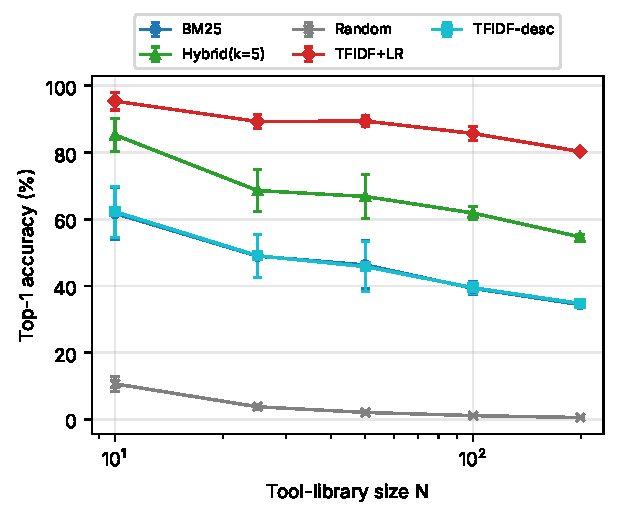
\includegraphics[width=\columnwidth]{figures/fig_e1_scaling.pdf}\caption{E1: top-1 vs.\ library size (mean $\pm$ s.d., 5 seeds). BM25 and TF-IDF-desc overlap.}\label{fig:e1}\end{figure}

\subsection{E2: unseen tools (RQ2)}
Table~\ref{tab:e2} shows that the supervised selector scores \TLRunseen\% on unseen tools. This is \emph{structural}: a classifier cannot output a class absent from training, so the result confirms the review's claim only trivially; the informative comparison is among retrieval methods. Description-only retrieval keeps \TTFdunseen\,$\pm$\,\TTFdunseenSd\% on unseen tools and \TTFdseen\% on seen tools; these two numbers are \emph{not} comparable (different tool subsets per seed, large s.d.), so they do not show that unseen tools are ``easier''. The paired comparison is within the same tools: Hybrid($k{=}5$) improves seen-tool accuracy from \TTFdseen\% to \THybseen\% and, perhaps surprisingly, unseen-tool accuracy by \PHybTFdunseen\,pp (s.d.\ \PHybTFdunseenSd, positive in \PHybTFdunseenPos/5 seeds). A plausible but \emph{untested} explanation is that lengthening other tools' documents with concrete queries changes term weights and reduces spurious matches to them. The sensitivity sweep (Fig.~\ref{fig:k}) shows seen-tool accuracy rising steadily with $k$ (\Kkzeroseen\% at $k{=}0$ to \Kktwentyseen\% at $k{=}20$) while unseen-tool accuracy moves only from \Kkzerounseen\% to \Kktwentyunseen\%. Appending tool-name tokens helped description-only retrieval on seen tools (\PTFnTFdseen\,pp, s.d.\ \PTFnTFdseenSd) and the effect on unseen tools was similar in mean but noisy (\PTFnTFdunseen\,pp, s.d.\ \PTFnTFdunseenSd).
\begin{figure}[t]\centering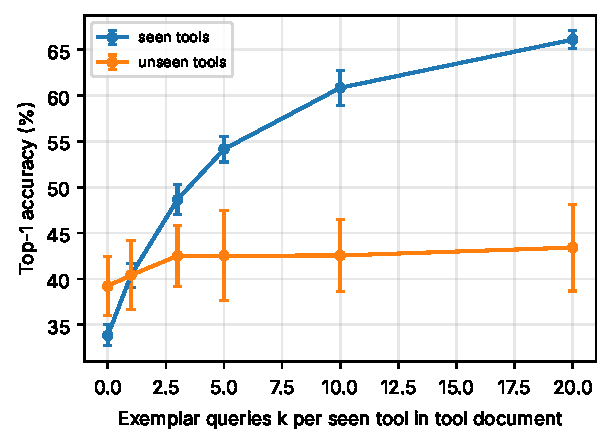
\includegraphics[width=\columnwidth]{figures/fig_e2_k_sweep.pdf}\caption{E2 sensitivity: exemplar queries per seen tool in the retrieval document (mean $\pm$ s.d.).}\label{fig:k}\end{figure}

\subsection{E3: abstention and EAS (RQ3)}
Fig.~\ref{fig:e3} and Table~\ref{tab:e3} give EAS. With $p_{out}{=}0.5$ and $c{=}1$, answering every query yields \SLRconepFiftyAll{} for the supervised model, \SHybconepFiftyAll{} for Hybrid and \SBMconepFiftyAll{} for BM25: \emph{all negative}, although each looks acceptable under accuracy. Rankings under EAS match the accuracy ranking whenever scores are non-negligible (answer-all at every $c$; abstention for $c\le2$: supervised $>$ Hybrid $>$ BM25 $\approx$ TF-IDF), so the review's implicit expectation that a cost-aware score would reorder systems is \textbf{not supported} here; what changes is the magnitude and sign. At $c{=}5$ with abstention every score is $\le$\,0.010 and the order among methods flips (Hybrid \SHybcfivepFiftyAbs{} vs.\ supervised \SLRcfivepFiftyAbs), a difference too small to interpret. Validation-tuned abstention recovers positive scores (supervised, $c{=}1$: \SLRconepFiftyAbs) by answering \SLRconepFiftyCovIn\% of in-library but still \SLRconepFiftyCovOut\% of out-of-library queries, with selective accuracy \SLRconepFiftySel\% on the answered in-library ones. Confidence separates the two groups only moderately (AUROC: BM25 \ABM, TF-IDF \ATFd, Hybrid \AHyb, supervised \ALR; s.d.\ \ABMSd--\AHybSd). At $c{=}5$ the benefit nearly vanishes (supervised abstain EAS \SLRcfivepFiftyAbs): the few out-of-library answers cancel the gains. The result depends strongly on $p_{out}$: at $p_{out}{=}0.1$, $c{=}1$ the supervised model scores \SLRconepTenAll{} when always answering and \SLRconepTenAbs{} with abstention. Because the out-of-library queries are queries whose gold tool exists but is withheld, this is a proxy for ``no suitable tool'', not MetaTool's own awareness task.
\begin{figure*}[t]\centering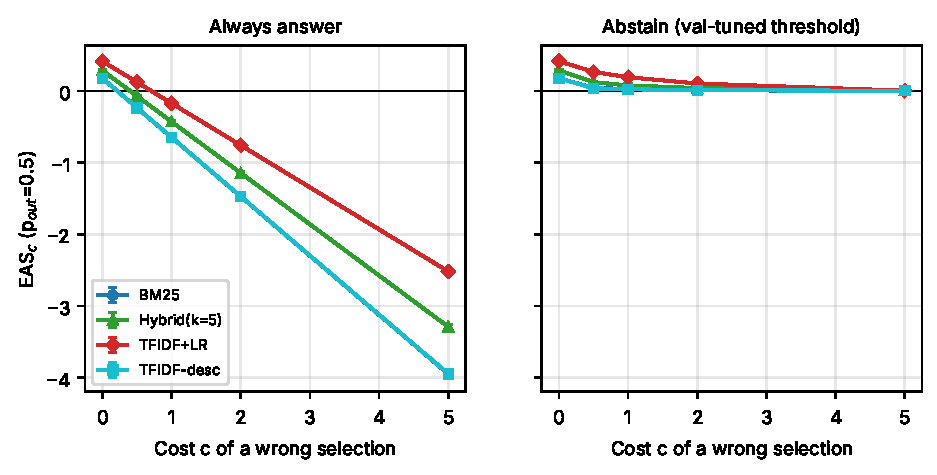
\includegraphics[width=0.78\textwidth]{figures/fig_e3_eas.pdf}\caption{E3: EAS$_c$ vs.\ cost of a wrong selection (mean $\pm$ s.d.\ over 5 seeds; BM25 hidden behind TF-IDF-desc).}\label{fig:e3}\end{figure*}

\subsection{Error and efficiency analysis}
For the supervised model, \XLRTopShare\% of its \XLRErr{} pooled errors fall in just 20 (gold,predicted) tool pairs (BM25: \XBMTopShare\%), mostly semantically adjacent tools (Table~\ref{tab:conf}: research-paper helpers, trip advice vs.\ trip tools, house renting vs.\ purchasing, two QR-code generators). Many such errors are arguably label ambiguity rather than method failure; I did not manually adjudicate them. Per-tool accuracy is only weakly related to training-set size for the supervised model (Spearman \XLRSpear). Accuracy is lowest on the longest queries ($>$40 words) for all methods (\texttt{results/error\_analysis.json}). Table~\ref{tab:eff} shows that all methods answer in about a millisecond or less on one CPU thread, but the supervised model needs \FLRFit\,s to train versus \FHybFit\,s to index; adding a new tool to a retrieval index takes at most \FHybFit{}\,s while the supervised model needs retraining and cannot select it before it has training queries.

\section{Discussion and Limitations}\label{sec:limits}
\textbf{What the evidence supports.} Selection accuracy of simple selectors degrades with library size; description matching alone is weak on this benchmark; a handful of exemplar queries per tool helps seen tools substantially and unseen tools slightly; accuracy alone hides the cost of wrong selections. \textbf{What it does not support.} Nothing here shows how LLMs behave: the review's claims about context limits and LLM hallucination remain \textsc{unknown} in this study. TF-IDF/LR on LLM-generated, template-like queries probably overstates the supervised model's advantage because training and test queries are close paraphrases of one another. Lexical retrieval is a floor, not a statement about dense retrievers. \textbf{Threats to validity.} (i)~One dataset whose queries and labels are LLM-generated; (ii)~near-duplicate tools make ``gold'' ambiguous; (iii)~library subsets are random and not nested; (iv)~only five seeds, no multiple-comparison control, and bootstrap intervals ignore tool-level dependence; (v)~$p_{out}$ and cost values are illustrative, not measured; (vi)~out-of-library queries are a proxy; (vii)~timing is from a single shared 1-vCPU machine. \textbf{Follow-ups (ranked by information per cost).} (1)~dense-embedding retrievers and a cross-encoder re-ranker on the same splits; (2)~an LLM selector under the same protocol with truncated vs.\ retrieved candidate lists; (3)~MetaTool's explicit no-tool queries to replace the withheld-tool proxy.

\section{Conclusion}
Under a frozen protocol on MetaTool, simple selectors lose accuracy as libraries grow, a supervised selector cannot handle new tools by construction while exemplar-augmented retrieval partly can, and a cost-adjusted score changes the \emph{sign} of deployable value rather than the \emph{ranking} of methods. Answering ``how well does an LLM agent select tools'' needs LLM experiments, which remain future work.

\paragraph{AI-use disclosure.} An AI assistant (Claude, Anthropic) was used for experiment design suggestions, code generation, debugging, analysis scripts and drafting. All reported numbers come from the code in the repository; see \texttt{ai\_assistance\_log.md} for the human verification record.

\bibliographystyle{unsrt}\bibliography{refs}
\end{document}
